\documentclass[a4paper,11pt]{article}
\usepackage{amsmath} % Advanced math typesetting
\usepackage[T1]{fontenc}
\usepackage[utf8]{inputenc} % Unicode support (Umlauts etc.)
\usepackage{lmodern}
\usepackage[english]{babel}  % Change hyphenation rules
\usepackage{authblk}
\usepackage{ragged2e}
\usepackage{graphicx}

\usepackage[
    sorting=none]{biblatex}
\DeclareCiteCommand{\supercite}[\mkbibsuperscript]
  {\iffieldundef{prenote}
     {}
     {\BibliographyWarning{Ignoring prenote argument}}%
   \iffieldundef{postnote}
     {}
     {\BibliographyWarning{Ignoring postnote argument}}}
  {\usebibmacro{citeindex}%
   \bibopenbracket\usebibmacro{cite}\bibclosebracket}
  {\supercitedelim}
  {}
  
  
%\usepackage[backend=biber,style=verbose-trad2]{biblatex} % Use biblatex package
\addbibresource{Bibliography/ACSEL_bibliography_1.bib}
%\bibliography{Bibliography/ACSEL_bibliography_1.bib} % The name of the .bib file (name without .bib)
\let\cite=\supercite

% Main document
% ---

\begin{document}
\title{%A quick overview on Floating Point and Monte Carlo arithmetics litterature -\\
Study of random rounding scheme applied to gradient descent method and Deep Neural Networks}
\author[1]{Christophe Pont}
\author[1]{David Defour}
\author[2]{Bijan Mohammadi}
\affil[1]{LAMPS, Univ. de Perpignan, 52 Av. Paul Alduy, 66860 Perpignan, France
\{christophe.pont,david.defour\}@univ-perp.fr}
\affil[2]{IMAG, Université de Montpellier, Place Eugène Bataillon, Montpellier, France.
bijan.mohammadi@umontpellier.fr}
\date{\today{}} % You can remove \today{} and type a date manually
\setcounter{Maxaffil}{0}
\renewcommand\Affilfont{\itshape\small}

\maketitle{} % Generates title
% FIXME passer à un anglais plus "simple" et épuré
\begin{sloppypar} \hspace{0pt} \\
  \begin{abstract}
    In this paper, we propose to explore the vast literature adressing the concerns raised by floating point arithmetic computations. We also introduce the reader to Monte Carlo Arithmetic (MCA)\cite{Parker1997}, a promising extension of floating point arithmetic. MCA exploit randomness in floating point computations in order to analyze and estimate the quality of numerical results.\\
    \indent Lastly, we extend this work in applying the {\ttfamily round\_random\_nearness} rounding method,
     giving an insightful trail on its use and performance on various gradient descent methods such as Krylov's conjugate gradient methods. 
    We also experiment its properties during stochastic gradient descent method, in the context of Deep Neural Network (DNN) training.
    %\begin{center}
    %This document aim to sum up my work during my thesis \emph{Improving trust in coastal erosion numerical simulations} and to keep track of my progress.
    %\end{center}
  \end{abstract}
\end{sloppypar}

%\newpage
\tableofcontents{} % Generates table of contents from sections
%\newpage

\section{Introduction}
%TODO Intro - Expliquer pourquoi on fait ça
%\par
\begin{sloppypar} \hspace{0pt} \\
\indent In order to fit real numbers into a finite number of bits, it is necessary to \emph{round} them. As one may already know though, this rounding can cause a loss of information, through loss of significant digits. Plus, each floating-point operation is followed by a rounding at the current precision, meaning potentially loosing information again. These undesired side-effects are called \emph{roundoff errors}\cite{kaneko1973local}. Numerical analysis aim at estimate this kind of errors in computations\cite{Hazewinkel1994}. As the number of operation grows, the cumulated errors eventually get worse; hence the issue of numerical reliability in large simulations. \\
\indent Among the various error sources, we propose to focus on roundoff errors, and more specifically to dig into the different rounding modes and their impact on the computations accuracy.\\
%   \\\emph{Briefly explain how floating point arithmetic can cause precision loss, and loss in reliability in the models and so fourth ==> reason of this paper}
\indent We study a rounding mode potentially able to \emph{balance} the precision loss of floating point computations, and displaying interesting properties: the \emph{stochastic rounding mode}. Parker previously called it the {\ttfamily round\_random\_nearness}\cite{Parker1997} rounding method. It rely on Monte Carlo Arithmetic to introduce randomness in roundings. %% Thus, the rounding method have zero expected error.
\end{sloppypar}
\begin{itemize}
  \item We propose to explain it and apply it to precision dependent contexts, and more precisely during gradient descent methods, particularly because they are vastly used during Deep Learning processes. Indeed, Deep Learning has seen a rise of interest since the applications of Deep Neural Networks (DNN). One of the learning method used is gradient descent method, thus it seems reasonnable to apply our findings to this field, as we'll see in the last part. %\emph{TODO : explain why deep learning is important (and therefore the value of this paper)?} % TODO describe how the field is important
  \item We expect to see the minimum precision required to converge increase as we use the stochastic rounding mode, hence having a reduced precision requirement for some memory expensive iterative process. % change it to "we prove that ..." when we have the results
\end{itemize}

\section{State of the art} % Background, concepts
\subsection{Floating point arithmetic}
\begin{itemize}
  \item Floating point arithmetic can be seen as a way for a physical computer to deal with theoretically infinitely many digits real numbers, given their finite physical memory capacity. To accomplish that, a real number is necessarily rounded to the closest floating point value (hence loosing part of the significant digits of the real number).
  \item Let's examine the basis of floating point numbers representation. \\ As Goldberg\cite{Goldberg1991} describes it, a floating point number of precision $\mathit{p}$, exponent $\mathit{e}$ and in base $\beta$ can be represented as such : $ \pm \mathit{d.dd\cdots d \times \beta^{e}} $. Here, $\mathit{d.dd\cdots d}$ is the significand of the floating point number, each $\mathit{d}$ being a distinct digit in base $\beta$; in other words \[ \forall \mathit{t} \in \left\lbrace 0,1\cdots p-1 \right\rbrace, \; 0 < \mathit{d}_{t} < \beta. \]
  \item The represented number is
  \begin{equation}
  %\[ 
  \pm \left( \mathit{d}_{0} + \mathit{d}_{1} \beta^{-1} + ... + \mathit{d}_{p-1} \beta^{- \left( \mathit{p} - 1 \right)} \right) \beta^{e}.  
  %\]
  \end{equation}
  \item The vast litterature\footnote{For the reader who'd like to dive deeper into the concepts stated here, Goldberg's\cite{Goldberg1991} tutorial form a great starting point.} 
  about the different kind of errors and their consequences tells us a lot about the gravity of these matters. 
  \item Cancellation errors arise when two close floating point number are substracted to one another, resulting a loss of significant digits. \emph{example} 
  %\emph{/!/ Basis of floating point arithmetic. A real number is approximated with the closest floating point value.}
  \item The different errors can accumulate and progressively drift the resulting value away from the real value it is supposed to describe % describe relative error?
  \item More recent approaches study the interesting properties of the application of Monte Carlo techniques to floating point arithmetic\cite{Parker1997}. MCA give us the ability to study the distribution of errors, through statistical analysis. It provides insightful quantification about roundoff errors and program instability. It also circumvent some anomalies of floating point arithmetic, as for instance the non associative summation (which is, with MCA, `statistically associative'.
  \item MCA approach has been the basis of numereous promising works, such as CADNA\cite{graillat2011stochastic} and Verificarlo\cite{denis:hal-01192668}.
\end{itemize}
\subsubsection{Rounding methods}
\begin{itemize}
  \item As seen earlier, when a real value isn't exactly representable as a floating point number, it is necessary to round it in order to store it in the computer's memory. 
  \item IEE754-1985 norm is a standard for floating-point arithmetic which adresses many problems found in previous implementations. It defines formats, operations and rounding rules in order to make the implementations more reliable and portable. The IEEE-754 norm suggest four rounding modes\cite{zuras2008ieee} :
  \begin{itemize}
    \item Round toward $0$
    \item Round toward $-\infty$
    \item Round toward $+\infty$
    \item Round to nearest (ties to even)
  \end{itemize}
  \item The most commonly used is round to nearest. However, it is does not come exempt of error\footnote{\emph{ref needed}}. MCA gives us two additionnal rounding modes : 
  \begin{itemize}
    \item {\ttfamily round\_random\_up\_or\_down} rounding method. It simply consists in rounding up or down with probability $\frac{1}{2}$
    \item {\ttfamily round\_random\_nearness} rounding method. In this case, the probability of rounding is related to the proximity of the corresponding floating point value. This is the rounding mode that give us the most promising results in our studied case. %TODO : find an example
  \end{itemize} % Stochastic rounding \emph{TODO explain its properties} %TODO explain the stochastic rounding properties
 % \\
 \end{itemize}
\subsection{Gradient descent methods}
\begin{itemize}
  \item We propose to apply this rounding mode to a specific iterative process : the conjuguate gradient method\footnote{A good introduction to this method can be found in the great related Shewchuk paper\cite{shewchuk1994introduction}.}. 
  \item The goal of the algorithm is to solve particular systems of linear equations (with a symmetric and positive-definite associated matrix).
  \item The conjuguate gradient method aim at solving linear equations systems, where the matrix is symmetric and positive defined. It iteratively minimize the function 
  \[ f : x \mapsto \frac{1}{2}\left(Ax,x\right)-\left(b,x\right) \] % TODO find a reference
  \item As we're about to see, its convergence is particularly sensitive to precision in floating point computations; hence also sensitive to the rounding mode used. % TODO find sources about this 
  %\emph{explain how it works and what it is used for. Plus why we're testing with it (because of the precision sensibility of the process}
\end{itemize}
\subsection{Deep Neural Networks, Learning Methods}
\begin{itemize}
   \item Deep Learning appear to benefit from a rise of interest, and many stunning industrial applications has emerged (especially from Google with DeepMind or Waymo\footnote{\emph{ref needed}}).
   \item Deep Neural Networks use different learning methods during inference phase; one of them is gradient descent method.
   \item In this context, studying the sensitivity of this method can give insightful perspectives. % TODO tellmemore
   \item Other works can give a good insight of the progress of this subject\cite{Gupta2015}\cite{Courbariaux2014}.
 \end{itemize} 


%\newpage
\section{Monte Carlo Arithmetic and stochastic rounding} % Method
\subsection{Method}
\emph{The method, why we chose it, which of its properties interest us...}
\\We decided to develop and validate the {\ttfamily round\_random\_nearness} method, and to apply it to a program of conjuguate gradient method (in $C$) with different parameters. % Present the context of the method, why we chose it, and which properties interested us. Also introduce the `matrice\_grad` program.}
\subsection{Tests}
\emph{Present the tests made to validate and prove our stochastic rounding mode. Why we are certain that it's working and some screenshots or tests results, with some examples showing its efficiency on simple cases}

\section{Results}
\subsection{Sensibility to rounding mode changes}
\begin{itemize}
  \item We applied this methodology to a conjuguate gradient descent method, by changing the precision used for each run, from 2 bits to 100. We then gathered the last value of the gradient after 60 iterations, and did it for each computed precision. 
  \item Below you'll see a plot showing the difference between the stochastic rounding and classic RNDN rounding. For now though, it looks like for lower precisions (<20 bits), both stochastic and RNDN diverge, and stochastic rounding seem to diverge a little bit more. They tend to converge from a precision of 25 bits, apparently in the same way. \emph{more tests will be made in order to test other data and to assert this result. Indeed, the randomness of our stochastic rounding is yet to be proven} % \emph{Experimenting sensibility of rounding mode changes + results }
%     \begin{figure}
% %     \begin{center}
%       \includegraphics[scale=0.26]{illustrations/stochastic.png}
%       \caption{Gradient descent with stochastic rounding}
%       \label{fig:}
% %     \end{center}
%   \end{figure}
% % 
\end{itemize}
  \begin{figure}[h]
    \begin{center}
      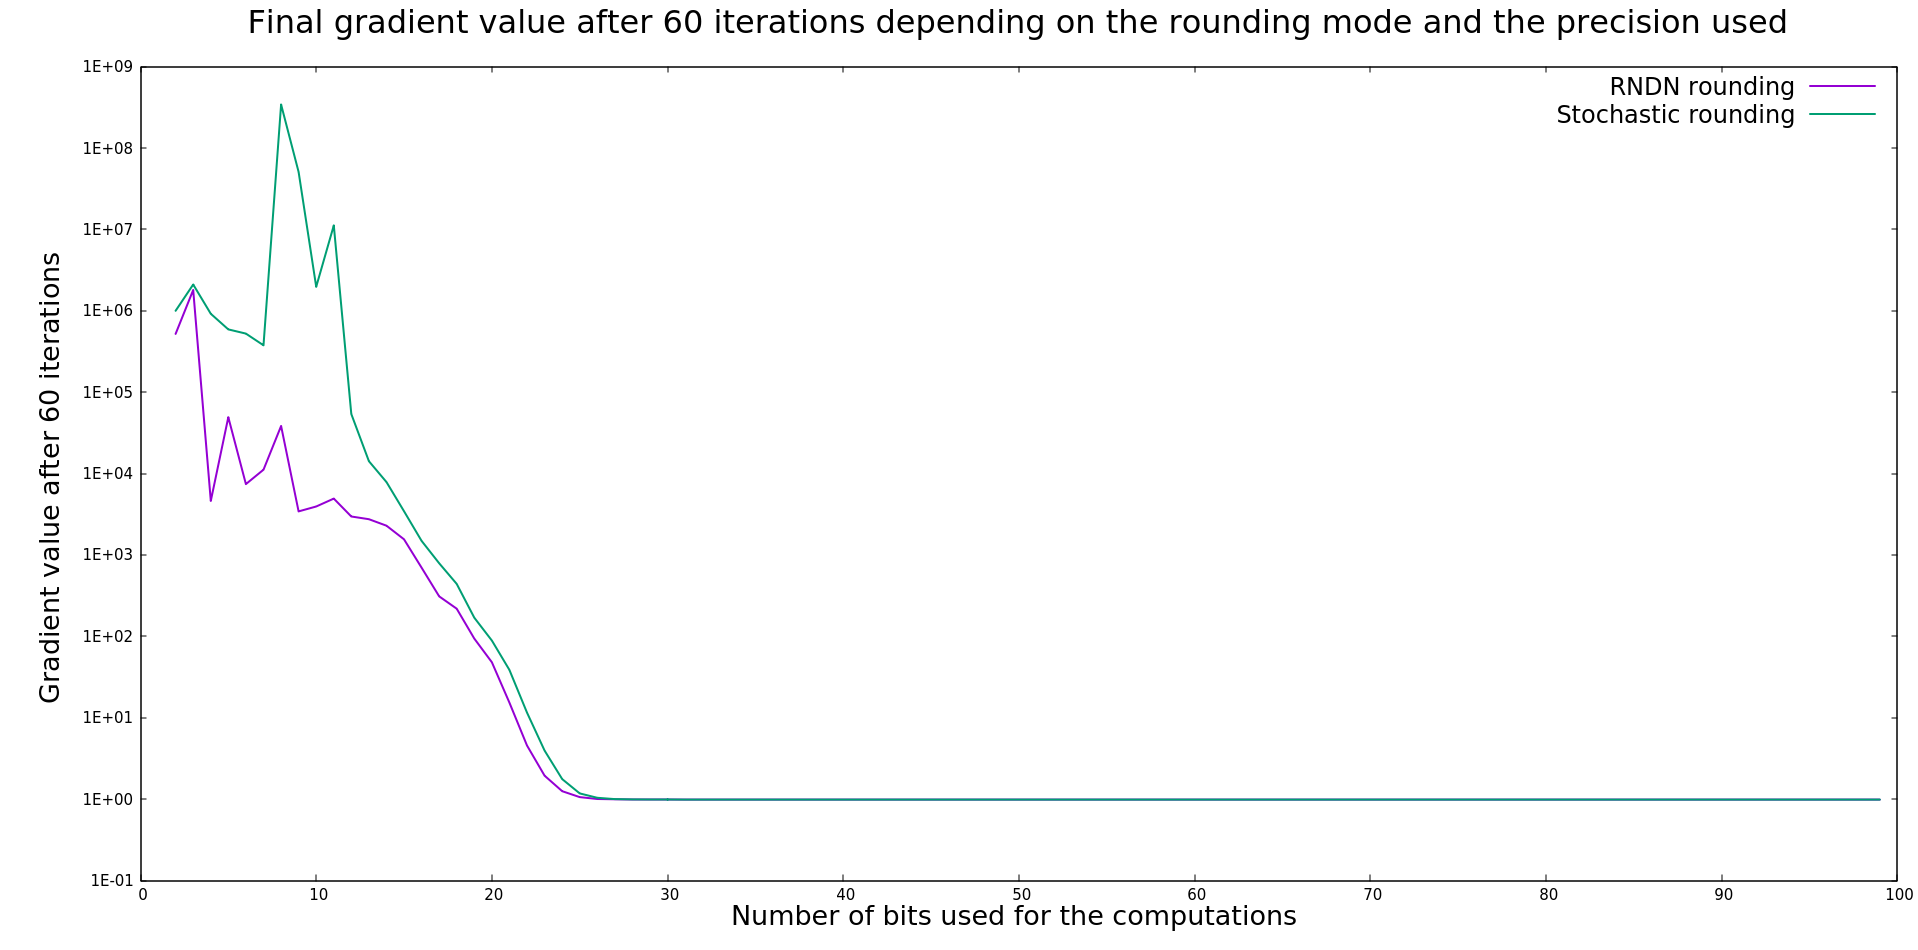
\includegraphics[width=1.1\textwidth,height=250pt]{illustrations/simple_comparison.png}
      \caption{First results}
      \label{fig:}
    \end{center}
  \end{figure}
  \begin{itemize}
  \item \emph{What is the impact of changing the rounding mode on \textbf{performance} and \textbf{reliability} (in what way this change implies a deviation on \textbf{convergence}) }
  \item \emph{resulting tables and charts of precision level for each configuration}
\end{itemize}

\subsection{Other experimented sensibilities}
\emph{
Results of varying:
\begin{itemize}
  \item the matrix size,
  \item the matrix type,
  \item the number of iterations,
  \item the random repartition function of the stochastic rounding
  \item and the floating point numbers precision
\end{itemize}
with results associated if relevant}

%\newpage
\section{Conclusion and future works}
\begin{itemize}
  \item \emph{Conclude about our approach, our results, and if needed the other thing that could need to be done}
  \item \emph{Cite other similar initiatives, such as Precimonious\cite{Rubio-Gonzalez2013} or Verrou\cite{fevotte2016verrou}.}
\end{itemize}


%\subsection{Random rounding in stochastic gradient method - Efficiency on Deep Neural Networks}
%Extending Gupta\&Al\cite{Gupta2015} and Courbariaux\cite{Courbariaux2014} works.

\newpage
\printbibliography

\end{document}
